\documentclass[a4paper]{exam}

\usepackage{epigraph} 
\usepackage{graphicx}
\usepackage{hyperref}
\usepackage{pythonhighlight}

\title{Weekly Challenge 09: Pathfinding}
\author{CS/CE 412/471 Algorithms: Design and Analysis}
\date{Spring 2025}

\begin{document}
\maketitle
\thispagestyle{empty}

\section*{Purpose}

In this WC, you will explore \textit{graph-based pathfinding} using \textit{breadth-first search (BFS)} and \textit{depth-first search (DFS)}. You will implement these algorithms to find paths in a randomly generated maze-like graph, and visualize the search process. This task will deepen your understanding of \textit{graph traversal techniques} and \textit{visualization in Python}, skills that are essential in fields such as \textit{AI, robotics}, and \textit{network analysis}.

\subsection*{Skills}

This WC builds your skills in computational problem-solving, algorithmic reasoning, and graph algorithms and efficient search strategies. These align with the university's  \href{https://habib.edu.pk/about-us/vision-values/}{learning goals}, the CS program's \href{https://habib.edu.pk/academics/sse/computer-science/}{learning outcomes}, and the course's \href{https://hulms.instructure.com/courses/4297/outcomes}{learning objectives}.

Problems similar to the one described in this WC arise commonly in game development, shortest path problems, network routing, and AI-driven decision-making.

Applying computer science concepts and computational thinking to real world problems in this manner will make you a more capable and versatile computer scientist.

Specifically, this WC develops expertise in:
\begin{itemize}
\item Algorithm Design and Analysis: implementing and comparing BFS and DFS for pathfinding.
\item Graph Representation and Manipulation: using \pyth{networkx} to construct and modify graph structures
\item Visualization and Animation: utilizing \pyth{matplotlib} to visualize search strategies step by step.
\item Problem Solving: analyzing and debugging pathfinding behavior in randomly generated mazes.
\end{itemize}

\section*{Background and Requirements}

To attempt and submit the WC, you will require:
\begin{itemize}
\item Understanding of graph properties such as connectivity and adjacency.
\item Knowledge of BFS and DFS algorithms
\item The ability to apply algorithmic thinking to solve a problem
\item The ability to program in Python and to read and follow technical tutorials
\item Experience with the \pyth{networkx} and \pyth{matplotlib} packages for working with graphs and generating visualizations.
\item Ability to structure and modularize code for readability and debugging.
\end{itemize}
\newpage

\epigraph{A dead end is just a good place to turn around!}

\noindent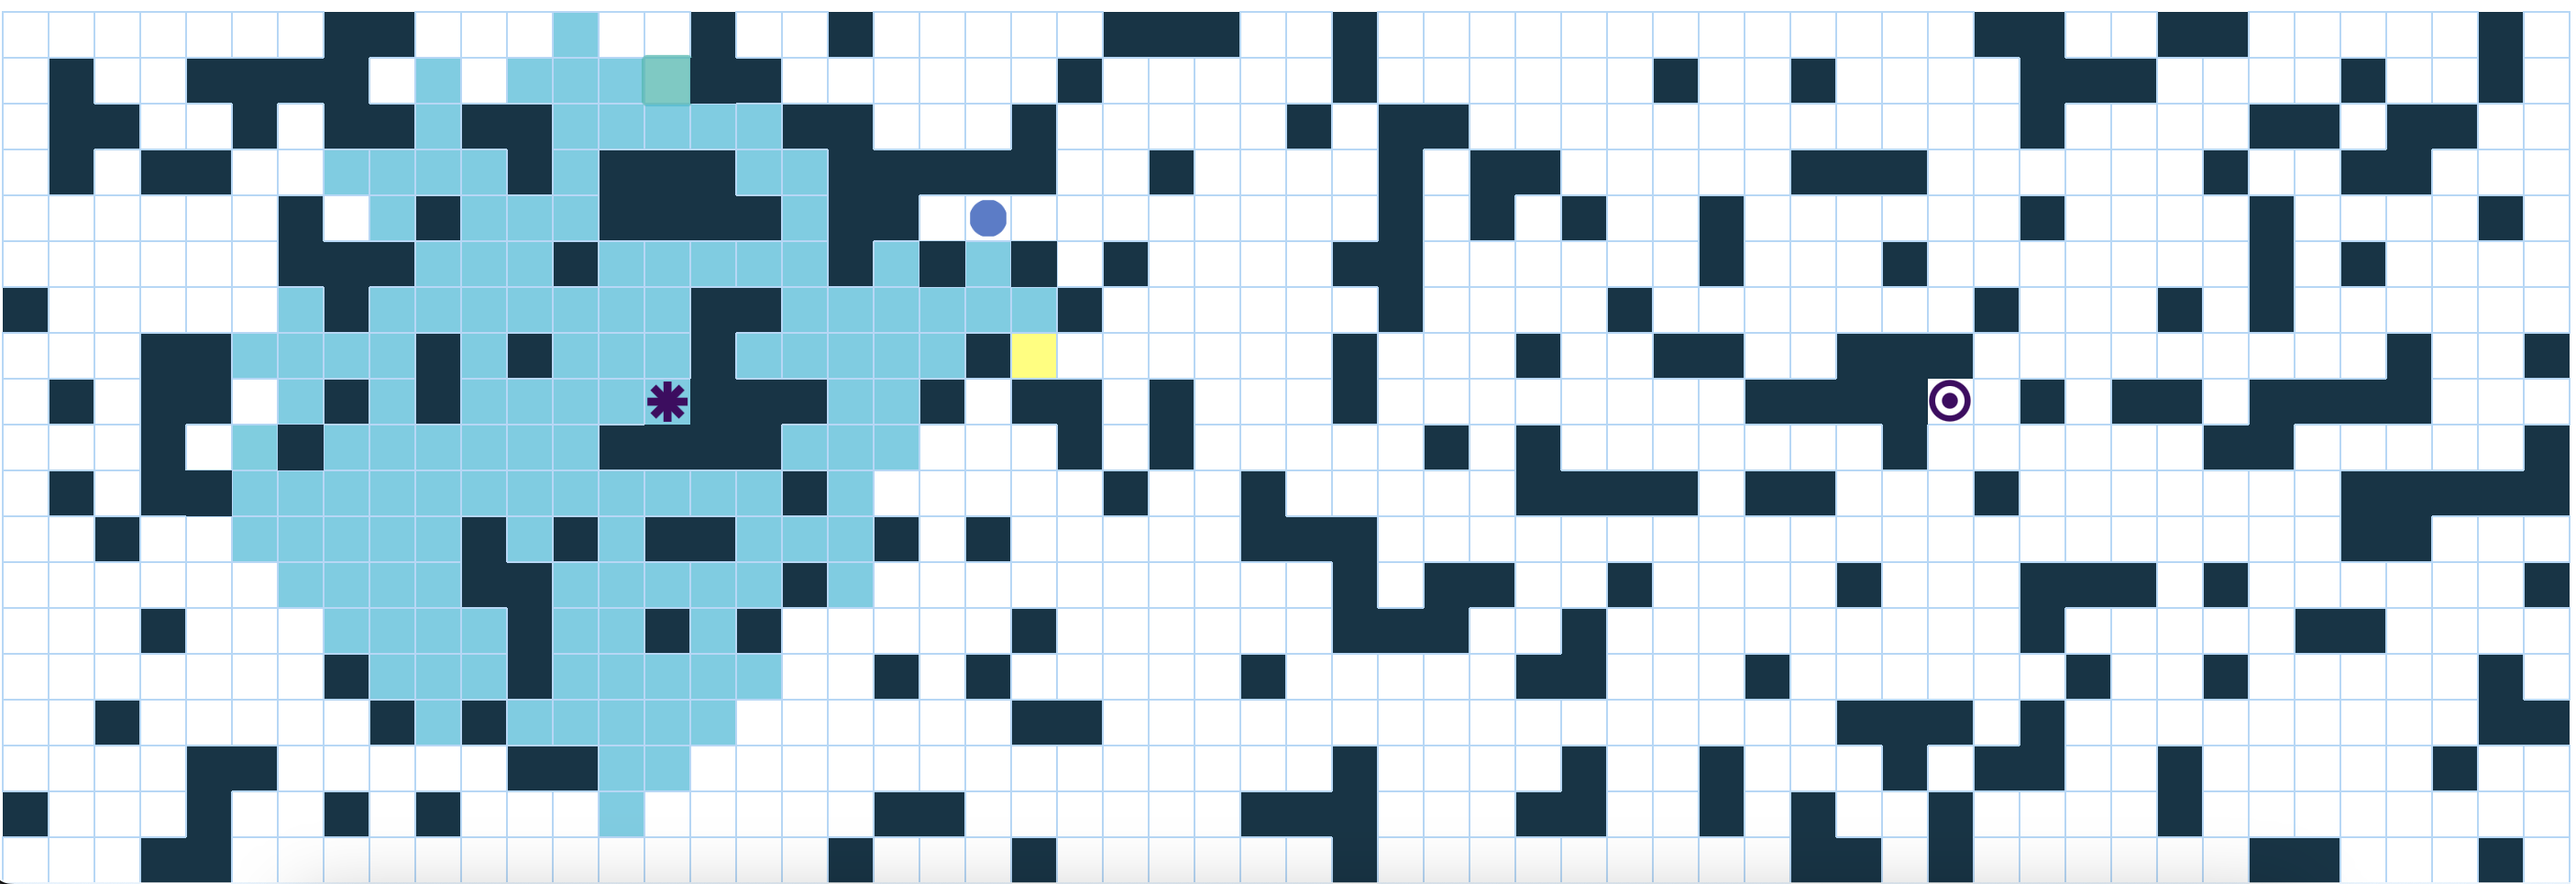
\includegraphics[width=\textwidth]{search}

Graphs are a popular structure in computer science and many types of graphs have been defined. For example, \href{https://networkx.org/documentation/stable/reference/generators.html}{a wide variety} is provided by the \pyth{networkx} package in Python.

We are going to consider a graph as a maze. Nodes represent positions and each egde represents a valid move from one position to another. Randomly assigning one node as the source and another as the destination, we will use two different strategies to find a path from the source to the destination. We will visualize each of the search strategies through an animation by coloring the source and destination nodes, the nodes considered in the search, and, finally, the nodes in the discovered path.

\section*{Tasks}

You will have to choose a graph to serve as your maze. Visualize different graph types from the \href{https://networkx.org/documentation/stable/reference/generators.html}{\pyth{networkx} package} in Python in order to finalize one that is to your satisfaction.

Once you have chosen your graph, you have to write a program to perform the following tasks.
  \begin{enumerate}
  \item Initialize your graph. If the graph is \href{https://mathworld.wolfram.com/ConnectedGraph.html}{connected}, then randomly remove some edges, e.g., by generating a random number, $z_i$, in $[0,1]$ at each edge, $e_i$, and deleting $e_i$ if $z_i$ is below some predefined probability, $p$. The resulting graph must have a reasonable number of nodes (at least 20) and edges (at least 50).
  \item In your graph, randomly assign one node as the source and another as the destination. Make sure that the nodes are not \href{https://en.wikipedia.org/wiki/Vertex_(graph_theory)#Types_of_vertices}{isolated}.
  \item Use breadth-first search to find a path from the source node to the destination node. The path is found and the search terminates when the destination node is visited for the first time. You will have to keep track of the visited nodes and of the discovered path for your visualization which is defined below.
  \item Use depth-first search to find a path from the source node to the destination node. The path is found and the search terminates when the destination node is visited for the first time. You will have to keep track of the visited nodes and of the discovered path for your visualization which is defined below.
  \item Visualize your search as an animation as follows. Each frame of the animation shows your maze and a step of your search. In the first frame, the source and destination nodes are visualized in different colors and the search is about to commence. In each step, depending on the current strategy, the search visits a new node or backtracks from a visited node. The search terminates when the destination is visited and the search is successful or no further nodes can be visited and the search has failed. In case of a successful search, color the nodes on the path from the source to the destination.
  \end{enumerate}

\section*{Example}
See the \href{https://clementmihailescu.github.io/Pathfinding-Visualizer/#}{Pathfinding Visualizer} as an example. The animation has more features than required for this WC. For example, it is grid-based whereas we are using a graph, visited nodes change shape and color whereas ours will retain their shape and only get colored one during the search, etc.

\section*{Hints}
Use the \texttt{matplotlib} package for visualization and saving animations as in previous WCs.


\section*{Submission}
You will submit
\begin{itemize}
\item your python file:
  \begin{itemize}
  \item Make sure that it only \pyth{import}s built-in packages, \pyth{networkx}, and \pyth{matplotlib}.
  \item Ensure a global variable, \pyth{STRATEGY}, at the top of the file that can be set to \pyth{BFS} or \pyth{DFS} to decide the strategy.
  \item Ensure a global variable, \pyth{SAVE}, at the top of the file. When \pyth{True}, running your python script will save the animation to a file \texttt{search.mp4}, otherwise the animation is launched on the desktop.
  \end{itemize}
\item an MP4 file, \texttt{bfs.mp4}, showing a breadth-first search. 
\item an MP4 file, \texttt{dfs.mp4}, showing a depth-first search. 
\end{itemize}

\end{document}

%%% Local Variables:
%%% mode: latex
%%% TeX-master: t
%%% End:
